%Thys Meintjes for M.Eng 
%introduction.tex
%included in skripsie.tex


\section{Rationale}

The electroencephalogram (EEG) is a recording of the gross electrical
activity of the brain as measured on the scalp surface. The EEG signal
measured between points on the scalp is the sum of all neuronal
electrical activity in the vicinity of the measuring electrode
conducted to the area where the electrode resides.

The aim of brain research and the subsequent recording of EEG signals
is to understand the relationship between human brain activity and
human perception, cognition and goal directed action
\cite{human}. Various techniques involving stimulated brain responses
are routinely applied in clinical practice and research
environments. These include visual, audio and tactile evoked
potentials. Of these the visual evoked potential is the most widely
used and best understood phenomenon. Diagnostic techniques have been
developed using the visual evoked potential as primary investigative
tool.

The EEG can be used as a parameter in clinical practice for the
analysis and diagnosis of various central nervous system related
pathologies in both human and animal subjects. Electroencephalograms
are used in neurology and psychiatry, mainly to help diagnose diseases
of the brain, such as epilepsy (convulsions caused by a chaotic
activity of neurons), sleep disorders and brain
tumors\footnote{http://www.epub.org.br/cm/n03/tecnologia/eeg.htm}. Knowledge
obtained from EEG data is of a phenomenological nature and usually
relies on the visual analysis of a EEG.

The exact source of various EEG signal artifacts is a subject of
continuous investigation.


In order to measure Bio-electric signals it is necessary to use
electrodes. EEG's are traditionally obtained by using standard gold or
silver surface electrodes with a conductive paste. Since the human
skin resistance varies between 10-100~k$\Omega$
\cite{active-electrode-ca} the potential derived with traditional
surface electrodes is affected by the electrode-skin resistance. The
main cause of skin resistance is the stratum granulosum layer forming
the human skin surface. In order to reduce skin resistance the stratum
granulosum is usually removed with a abrading paste. A conductive
electrode paste is applied to ensure a stable low impedance conductive
path between the electrode and skin surface.

Most recording artifacts and loss of data are directly attributed to
problems associated with the electrode and its application. By
negating the voltage dividing effect of the skin surface the need of a
low-impedance signal path and the associated preparation phase is
circumvented. The effect of skin resistance is negligible if the
electrode input impedance is significantly larger than the skin
resistance. This condition can be satisfied by using a active device
in the realization of the electrode. By replacing the traditional wet
electrodes with dry active electrodes the process of skin preparation
can be eliminated. Eliminating skin preparation and the need for
electrode paste significantly enhances the usability and ergonomic
acceptability of a EEG data acquisition system.


The successful elimination of the time and comfort constraints
introduced by traditional EEG electrode preparation and application
suggests various new application fields. Possible applications range
from enhanced computer interface designs to direct applications in the
rehabilitation engineering field such as appliance control interfaces
for the physically disabled.


\section{System overview}
This report documents the design and implementation of a active
electrode based EEG data--acquisition system. The system forges a path
between the opposing constraints of user--friendliness and signal
quality. This contention exists primarily due to the fact that
extensive skin preparations are needed before EEG recordings may be
attempted.

The author will attempt to demonstrate that the traditional
preparation phase may skipped without adversely affecting EEG signal
quality by applying active electrodes in stead of traditional passive
electrodes.


\begin{figure}[h]
		\psfrag{Signal}[][]{Signal}
		\psfrag{Acquisition}[][]{Acquisition}
		\psfrag{low-level}[][]{Low-level}
		\psfrag{signal}[][]{signal}
		\psfrag{processing}[][]{Processing}
		\psfrag{Conversion}[][]{Conversion}
		\psfrag{Display}[][]{Display}
		\psfrag{High-level}[][]{High-level}
        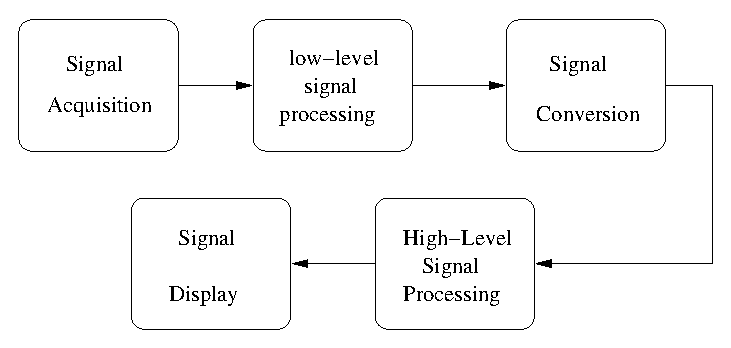
\includegraphics[width=\textwidth]{overview.eps} 
        \caption{System overview.}
        \label{fig:overview}
\end{figure}

Figure ~\vref{fig:overview} depicts the system as a logical and
physically separated set of five independent functional modules. Each
module is named according to its primary function:

\begin{itemize}
	\item{ A signal acquisition model containing a set of active
		  electrodes mounted on a adjustable head--band. This module
		  sets the system apart from more traditional EEG data
		  acquisition systems. [Chapter~\ref{chap:sa}].}
	\item{ A low--level signal processing module responsible for the
		  extraction and amplification of the EEG signal from the
		  acquired scalp signal. This module is implemented using
		  standard differential instrumentation amplifiers
		  [Chapter~\ref{chap:llsp}].}
	\item{ A signal conversion module used to digitize the extracted
          EEG signal [Chapter~\ref{chap:sc}].} This module is
		  implemented using of--the--shelf hardware and software.
	\item{ A high level signal processing module that allows for
	      specialized spectral processing and feature extraction
	      sub-modules [Chapter~\ref{chap:hlsp}].} This module is
		  implemented using commercial software. 
	\item{ A signal display module capable of displaying both the raw
		  EEG signal from the signal conversion module and the results
		  generated by the high--level signal processing module
		  [Chapter~\ref{chap:hlsp}].} This module is implemented using
		  standard PC hardware and commercial software.
\end{itemize}
	

Each module is designed and implemented with the reduction of
environmental and system noise as primary goal. Various techniques are
employed to prevent the degradation of the EEG signal by both external
interference and internal noise sources within each system module.


\section{General Specification}
\label{section:def-of-need}

Developing a set of definitive goals from a general specification
naturally leads toward and ultimately translates into a quantitative
system specification. Translating fuzzy concepts of
``user--friendliness'', ``ease--of--use'' and ``adequate signal
quality'' to measurable constants sets a qualitative standard against
which real progress and eventual system compliance may be evaluated.

\subsection{Terms and definitions}
\subsubsection{User--friendliness and ease of use}
User--friendliness and ease of use are qualitative ergonomic
specifications implying that the operator be allowed to achieve her
purpose with the minimum amount of system imposed constraints. This
includes among other things mobility constraints due to signal and
power cable lengths. The following quantitative values were chosen to
define ease of use and user--friendliness:

\begin{itemize}
	\item{Application and adjustment time: The maximum time spent to
	physically attach the active--electrode array - 10~s.}
	\item{Removal time: The maximum time spent removing the
	active--electrode array 5~s.}
	\item{Preparation time: Time spent to prepare the skin surface for
	the application of electrodes - none}
	\item{User discomfort: User discomfort is quantified as a function of
	the headband's weight and skin contact area. Acceptable values
	are: Weight 400~g, Contact Area 10~$cm^{2}$}
\end{itemize}

\subsubsection{Adequate signal quality.}
System signal quality is the underlying basis for the technical design
specification of the system and is the ultimate factor determining the
overall usability of the system. Signal quality is measured in terms
of the signal to noise ratio at the output of the signal conversion
module. The signal to noise ratio is defined throughout this document
as 20log10$(\frac{V_{s}}{V_{n}})$ with $V_{s}$ the EEG signal voltage
and $V_{n}$ the sum of all system and environmental noise
voltages. The minimum acceptable $S/N$ value is specified as
20~dB. The signal voltage must have a amplitude at least ten times the
noise voltage.

Table ~\vref{table:hl-design-contraints} summarizes the general
high-level system specification. 

\begin{table}
\begin{center}
\caption{High--level design constraints}
\label{table:hl-design-contraints}	
\begin{tabular}{|l|l|} 	\hline	
	Application and adjustment time & 10.0~s\\
	Removal time & 5~s\\
	Preparation time & 0~s\\
	Head--band Weight & 200~g\\
	Contact Area & 10~cm$^{2}$\\
	Signal conversion output minimum S/N & 20~dB \\\hline
\end{tabular}
\end{center}
\end{table}



\section{High level system specification}
\label{section:hl-system-specification}
In order to satisfy the conditions specified in the definition of need
(Section~\vref{section:def-of-need}) a top-down system design approach
is adopted leading to a modular system design. Modularizing the system
eases the testing and evaluation process significantly and allows the
design to budget for acceptable noise levels within the individual
modules. As noise added to the system by a module is cascaded into the
next module as part of the input signal it imperative that module
level noise sources be suppressed as far as possible. Adequate
screening is applied to limit the effect of environmental signal
contamination. Noise introduced by the environment will hence forward
be referred to as interference.


The system consists of several modules or sub--systems. The design
accommodates the whole measurement process in a modular environment
which is closely integrated but easily customizable to suit the needs
of a particular measurement. Each module in the system object diagram
is implemented and tested in isolation before being integrated with
the rest of the system. This process contributed to the need of a
standard test or measurement environment. The Standard measurement
environment (SME) is discussed in Chapter~\ref{chap:sme}.

\begin{figure}[htbp]
\begin{center}
        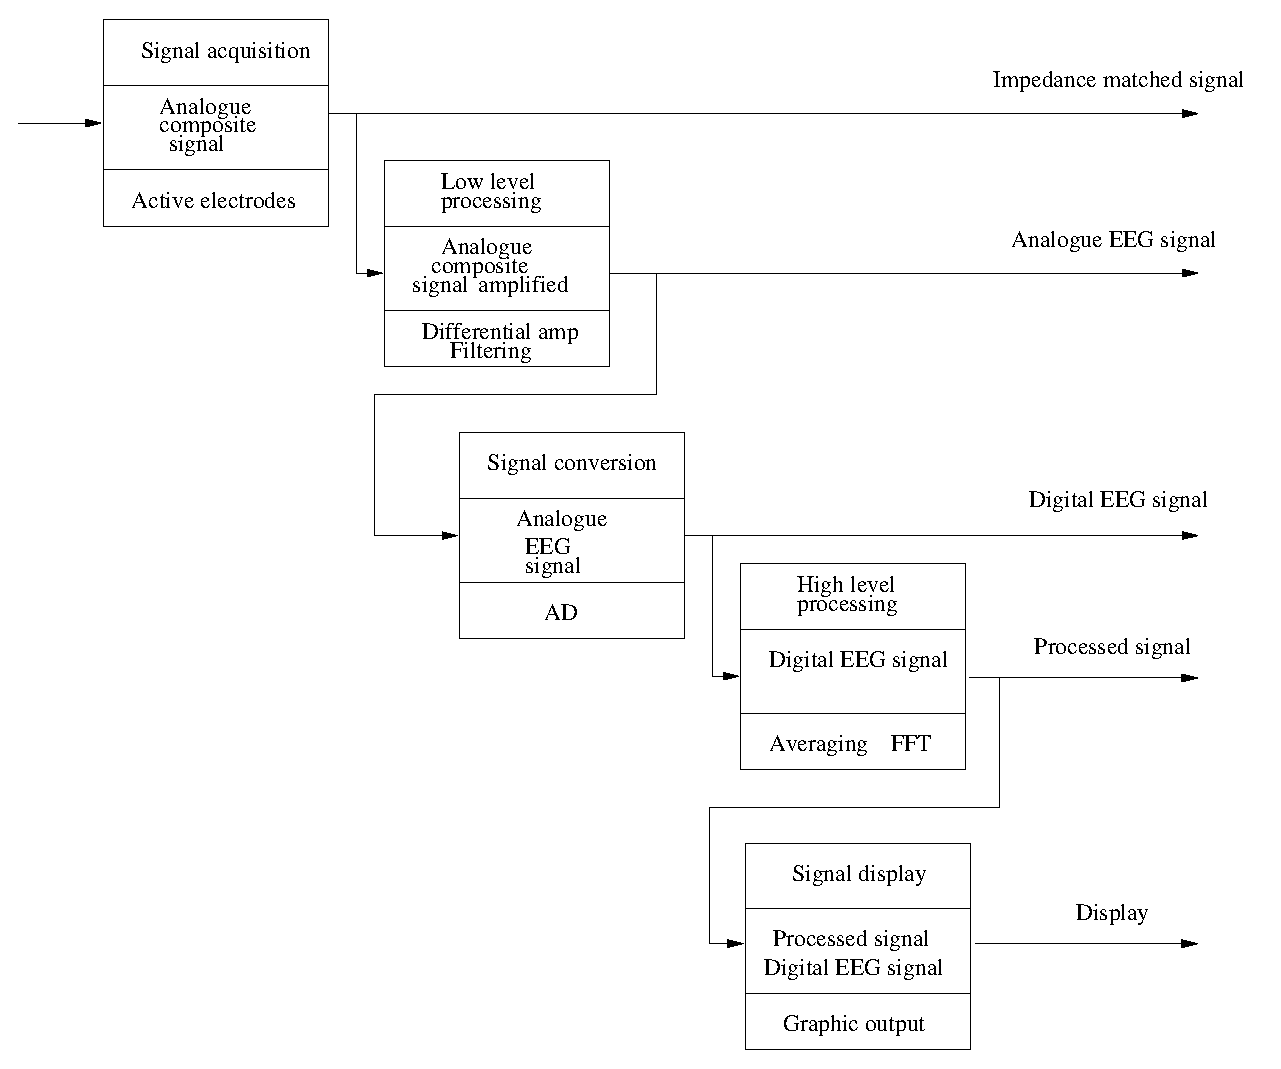
\includegraphics[width=\textwidth]{eeg-signal-flow.eps}
        \caption{System signal flow diagram.}
        \label{fig:eeg-signal-flow}
\end{center}
\end{figure}

The system signal flow diagram depicted in
Figure~\vref{fig:eeg-signal-flow} illustrates the flow of the EEG
signal through the system. The signal enters the system at the signal
acquisition module, moves through the various modules and ends up in
the signal display module.

The system consists of five distinct modules:

\begin{itemize}
	\item{Signal acquisition module. }
	\item{Low level signal processing module.}
	\item{Signal conversion module.}
	\item{High level signal processing module.} 
	\item{Signal display module.}
\end{itemize}

A brief description of each module follows. Each module has a chapter
dedicated to it and is discussed at length therein.


The \textbf{signal acquisition module} (SAM) acquires the EEG signal
from the scalp. The SAM module is the system's primary physical
interface with the user. The implementation of this module have to
comply to the prerequisites of weight and contact area specified in
the definition of need. This module makes use of a FET-driven
active--electrode array which reduces the severity many of the
problems associated with traditional electrodes. The electrode array
is implemented using low noise FET--input operation amplifiers. The
array is mounted on a user--adjustable head--band. The user may set
the pressure exerted by the metal conductors on the scalp to a
comfortable level by adjusting the head--band appropriately.


The \textbf{low--level signal processing module} (LLSPM) extracts,
amplifies and filters the EEG signal from the SAM output signal. The
LLSPM is a critical system module and is designed and implemented with
cognizance of noise contamination from external as well as internal
sources. Signal contamination concerns ensures that care is taken to
screen this module adequately. A shoddy implementation of a sound
design will render the system useless. Monolithic differential
amplifiers are used in this module as well as switched capacitor
filters. 


The \textbf{signal conversion module} (SCM) digitizes the analogue EEG
signal for further processing by the secondary signal processing
module. This module consists of a commercial analogue to digital (A/D)
system. Signal noise introduced by the conversion process is
considered to some degree in the SCM's design.

The \textbf{high level signal processing module} (HLSPM) is
responsible for complex signal manipulation. This includes averaging
and feature extraction modes. Real time as well as off--line
processing is possible. 


The \textbf{signal display module} (SDM) displays the results produced
by the HLSPM. This module is closely associated with the high level
signal processing module, the HLSPM is however not bounded to any
specific graphical interface. In compliance with the basic UNIX
philosophy of modularizing software the HLSPM and SDM are separate
packages. This enables a Internet--connected investigator to monitor
running experiments from any Internet access point. This module is
also implemented using custom made Linux based software and available
libraries.


\section{The standard measurement environment}
In order to test the various modules during the different stages of
system development and the system as a whole, a standard measurement
environment (SME) was developed and used. The SME consists of a
physical and electrical model of the human head and emulates the
signal conditions present at the scalp. The use of a standard
measurement environment makes the quantitative evaluation of a
module's performance with different configurations possible. The SME
is applied as a test bench and a rapid development tool throughout
the system design cycle.


\section{Report structure}
The design and implementation of each module is discussed in this
report. The general structure of this document follows the general
signal path of the EEG signal, as depicted in the signal flow diagram
of Figure~\vref{fig:eeg-signal-flow}. The design and implementation of
the standard measurement environment is discussed first as all other
modules were tested and developed using the standard measurement
environment.


The design specifications and implementation detail for a module is
discussed under that module's name as described in
Figure~\vref{fig:eeg-signal-flow} and
Section~\ref{section:hl-system-specification}. Secondary
considerations concerning the design and implementation of a specific
module are also included in the discussion when necessary. Appendices
are used when the subject matter warrants it.
























